\documentclass[aspectratio=169,11pt]{beamer}

% Shared style, ported from the UF Animal Sciences 2026 talk (ib-tutorials.sty at the repo root).
\makeatletter\def\input@path{{./}{../}}\makeatother
\usepackage{ib-tutorials}

\usepackage[utf8]{inputenc}
\usepackage{amsmath,amssymb,bm}
\usepackage{booktabs}
\usepackage{graphicx}
\usepackage{xcolor}
\usepackage{listings}
\usepackage{tikz}
\usetikzlibrary{arrows.meta,positioning,shapes.geometric,fit,calc}
\usepackage{hyperref}

\graphicspath{{pictures/planktos/}{../pictures/planktos/}}
\newcommand{\xx}{\bm{x}}
\newcommand{\XX}{\bm{X}}
\newcommand{\uu}{\bm{u}}
\newcommand{\bb}{\bm{b}}
\newcommand{\sourcecredit}[1]{\vfill\hfill{\tiny\textcolor{DarkGray}{#1}}}

% Listings in the talk palette: NavyBlue keywords, DarkGray italic comments,
% OliveGreen strings, light-gray panel with a hairline gray frame.
\lstset{
  basicstyle=\ttfamily\scriptsize\color{BlackGray},
  keywordstyle=\color{NavyBlue}\bfseries,
  commentstyle=\color{DarkGray}\itshape,
  stringstyle=\color{OliveGreen},
  showstringspaces=false,
  columns=fullflexible,
  keepspaces=true,
  frame=single,
  framerule=0.4pt,
  rulecolor=\color{LightGray},
  backgroundcolor=\color{LightGray!30},
  xleftmargin=0.25em,
  xrightmargin=0.25em
}

\title[What is Planktos?]{What is Planktos?}
\subtitle{Agent-based modeling in prescribed fluid flows}
\author[Miller]{Laura A. Miller}
\institute[UArizona]{Department of Mathematics, University of Arizona}
\date{Using IB Software \textbullet\ Planktos}

\begin{document}

% 1
\begin{frame}[plain]
% The central-idea panel and source line sit in the free right half below the title rule.
\begin{tikzpicture}[remember picture,overlay]
  \node[anchor=north east,text width=0.38\paperwidth,inner sep=0pt] at ([xshift=-5mm,yshift=-33mm]current page.north east) {%
    \begin{block}{The central idea}
      \small Move many autonomous organisms through a resolved velocity field while retaining behavior, stochasticity, and collision geometry.
    \end{block}
    \vspace{4pt}
    {\tiny\color{DarkGray}Source basis: Strickland et al. (2022), Hamlet et al. (2023), and Planktos commit \code{a1c2128} (2026-08-19).\par}};
\end{tikzpicture}%
\maketutorialtitle
\end{frame}

% 2
\begin{frame}{Learning goals}
By the end, you should be able to:
\begin{enumerate}
  \item state when a \textbf{one-way-coupled point-agent} model is defensible;
  \item map a scientific question to an \code{Environment} and one or more \code{Swarm} objects;
  \item choose among ODE, It\^o SDE, and custom algorithmic behavior;
  \item explain how Planktos interpolates flow data and enforces outer and immersed boundaries;
  \item distinguish trajectory visualization, KDE, and FTLE diagnostics;
  \item interpret the gorgonian capture example without overextending its assumptions.
\end{enumerate}
\end{frame}

% 3
\begin{frame}{The scientific problem: behavior inside transport}
\begin{columns}[T,onlytextwidth]
  \begin{column}{0.52\textwidth}
    \begin{itemize}
      \item Marine and aerial plankton are carried by spatially and temporally varying flows.
      \item They may also swim, fly, align, settle, search, or respond to environmental cues.
      \item Obstacles and living structures reshape the flow and create collision or capture surfaces.
      \item The observable is often a \textbf{distribution}: dispersal, residence, encounter, or capture probability.
    \end{itemize}
  \end{column}
  \begin{column}{0.46\textwidth}
    \centering
    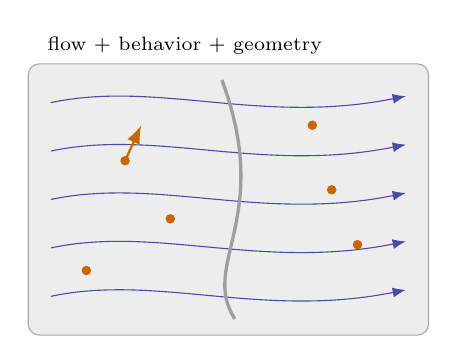
\begin{tikzpicture}[scale=0.82,>=Latex]
      \draw[rounded corners,fill=LightGray!40,draw=DarkGray] (0,0) rectangle (6.2,4.2);
      \foreach \y in {0.6,1.35,2.1,2.85,3.6}{
        \draw[->,NavyBlue!70] (0.35,\y) .. controls (2.0,\y+0.35) and (3.6,\y-0.35) .. (5.85,\y+0.1);
      }
      \draw[very thick,gray!75] (3.2,0.25) .. controls (2.65,1.1) and (3.8,1.8) .. (3.0,3.95);
      \foreach \p in {(0.9,1.0),(1.5,2.7),(2.2,1.8),(4.4,3.25),(5.1,1.4),(4.7,2.25)}{
        \fill[orange!80!black] \p circle (2.1pt);
      }
      \draw[->,orange!80!black,thick] (1.5,2.7) -- +(0.25,0.55);
      \node[anchor=south west,font=\scriptsize] at (0.15,4.2) {flow $+$ behavior $+$ geometry};
    \end{tikzpicture}
  \end{column}
\end{columns}
\sourcecredit{Scientific framing: Strickland et al. (2022), Sections 1 and 5. Schematic: instructor's course notes.}
\end{frame}

% 4
\begin{frame}{A competition of velocities and scales}
\begin{columns}[T,onlytextwidth]
  \begin{column}{0.55\textwidth}
    A useful first diagnostic is the velocity ratio
    \[
      V_r=\frac{U_a}{U_f},
    \]
    where $U_a$ is a characteristic active speed and $U_f$ is a characteristic ambient-flow speed.
    \begin{itemize}
      \item $V_r\ll1$: transport is mostly flow-driven.
      \item $V_r\sim1$: behavior and advection compete strongly.
      \item $V_r\gg1$: active motion may dominate locally.
    \end{itemize}
  \end{column}
  \begin{column}{0.43\textwidth}
    \begin{block}{Do not stop at one ratio}
      Also compare body size, obstacle spacing, correlation time, diffusivity, and observation time. $V_r$ organizes regimes; it does not prove that a point-agent or one-way coupling is valid.
    \end{block}
  \end{column}
\end{columns}
\sourcecredit{Velocity-ratio framing: Strickland et al. (2022), Section 1.}
\end{frame}

% 5
\begin{frame}{The modeling contract: one-way coupling}
\begin{block}{Assumption}
The flow and immersed geometry influence the agents, but the agents do not alter either one.
\end{block}
\begin{columns}[T,onlytextwidth]
  \begin{column}{0.48\textwidth}
    \textbf{Plausible when}
    \begin{itemize}
      \item agents are small relative to resolved flow scales;
      \item concentrations are low enough to neglect collective forcing;
      \item wakes and body-induced disturbances decay before affecting other agents;
      \item agent shape can be reduced to a point trajectory for the question asked.
    \end{itemize}
  \end{column}
  \begin{column}{0.48\textwidth}
    \textbf{Questionable when}
    \begin{itemize}
      \item dense suspensions actively mix the fluid;
      \item locomotion produces persistent wakes or stresses;
      \item deformable-body hydrodynamics controls motion;
      \item capture depends on unresolved finite-size contact physics.
    \end{itemize}
  \end{column}
\end{columns}
\sourcecredit{Scope and limitations: Strickland et al. (2022), Abstract and Section 5.}
\end{frame}

% 6
\begin{frame}{The point-agent equation}
One common model represented by Planktos is
\[
  d\XX_t=\big[\uu(\XX_t,t)+\bb(\XX_t,t,\mathcal S_t)\big]dt
  +\bm{\sigma}(\XX_t,t,\mathcal S_t)\,d\bm W_t.
\]
\begin{description}
  \item[$\uu$] prescribed fluid velocity, interpolated to the agent location;
  \item[$\bb$] active drift or deterministic behavior;
  \item[$\bm\sigma\,d\bm W_t$] stochastic motion, interpreted as an It\^o SDE by the built-in Euler--Maruyama route (the built-in solver restricts $\bm\sigma$; see the SDE slide);
  \item[$\mathcal S_t$] agent state, neighbor information, or other model variables supplied by the user.
\end{description}
\begin{alertblock}{Important}
This equation is a template, not a restriction: \code{apply\_agent\_model} may return positions from arbitrary code.
\end{alertblock}
\end{frame}

% 7
\begin{frame}{Nondimensional checks before simulation}
\begin{columns}[T,onlytextwidth]
  \begin{column}{0.52\textwidth}
    \begin{align*}
      V_r &= U_a/U_f,\\
      \mathrm{Pe} &= U_f L/D,\\
      \mathrm{St} &\sim \tau_p/\tau_f.
    \end{align*}
    \begin{itemize}
      \item $\mathrm{Pe}$ compares advective transport with diffusive spreading; $D$ is the agents' effective diffusivity (Planktos's covariance is $\texttt{cov}=2D$).
      \item A particle response-time ratio helps decide whether tracer dynamics are adequate: $\tau_p$ is the particle's viscous response time, $\tau_f=L/U_f$ the flow time.
    \end{itemize}
  \end{column}
  \begin{column}{0.44\textwidth}
    \begin{block}{Numerical resolution checks}
      \begin{itemize}
        \item Is $\Delta t$ small compared with flow and behavior time scales?
        \item Can an agent cross a thin obstacle in one step?
        \item Is the CFD mesh fine enough for the gradients the behavior uses?
      \end{itemize}
    \end{block}
    \begin{block}{Stokes number of a small sphere}
      \small For radius $a$ and $\tau_p=2a^2/(9\nu)$: $\mathrm{St}=\tfrac29(a/L)^2\mathrm{Re}$, $\mathrm{Re}=U_fL/\nu$, the form used by Planktos's inertial-particle model.
    \end{block}
  \end{column}
\end{columns}
\sourcecredit{$\mathrm{St}$ form: Haller \& Sapsis (2008), as implemented in \code{motion.inertial\_particles} (commit \code{a1c2128}).}
\end{frame}

% 8
\begin{frame}{What Planktos is---and is not}
\begin{columns}[T,onlytextwidth]
  \begin{column}{0.48\textwidth}
    \textbf{Planktos provides}
    \begin{itemize}
      \item vectorized 2D/3D agent simulation;
      \item prescribed steady or time-dependent velocity fields;
      \item ODE, It\^o SDE, and custom behavior routes;
      \item immersed-mesh collision handling;
      \item plotting, animation, KDE, vorticity, and FTLE tools.
    \end{itemize}
  \end{column}
  \begin{column}{0.48\textwidth}
    \textbf{Planktos does not}
    \begin{itemize}
      \item solve the Navier--Stokes equations;
      \item feed agent forces back into the flow;
      \item automatically validate biological assumptions;
      \item replace convergence, uncertainty, or sensitivity studies.
    \end{itemize}
  \end{column}
\end{columns}
\begin{block}{Current source audited for this tutorial}
Version 1.0.3, GPLv3, commit \code{a1c2128} (2026-08-19).
\end{block}
\end{frame}

% 9
\begin{frame}{Architecture: a world containing populations}
\centering
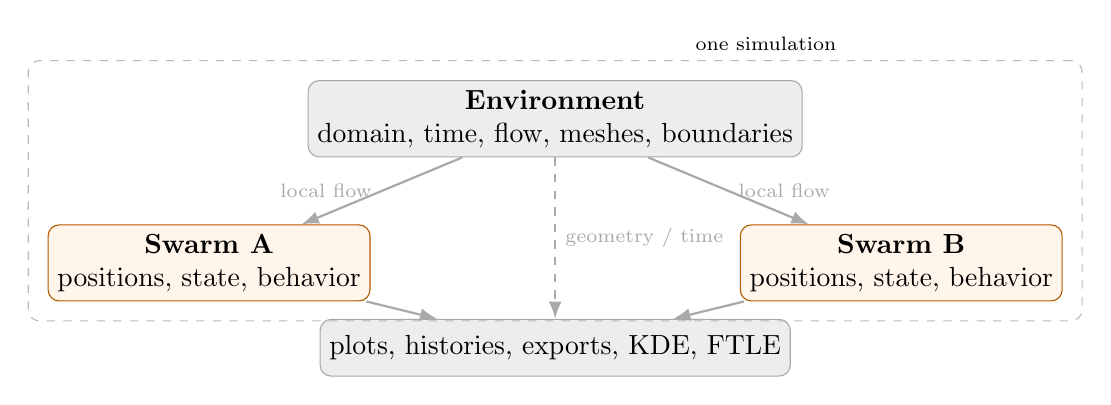
\begin{tikzpicture}[
  node distance=0.55cm and 1.05cm,
  box/.style={rounded corners,draw=DarkGray,fill=LightGray!40,minimum width=3.1cm,minimum height=0.72cm,align=center},
  sbox/.style={rounded corners,draw=orange!70!black,fill=orange!8,minimum width=2.8cm,minimum height=0.68cm,align=center},
  arr/.style={-{Latex[length=2.2mm]},thick,DarkGray}
]
  \node[box,minimum width=5.0cm,minimum height=0.85cm] (env) {\textbf{Environment}\\domain, time, flow, meshes, boundaries};
  \node[sbox,below left=0.85cm and -0.8cm of env] (s1) {\textbf{Swarm A}\\positions, state, behavior};
  \node[sbox,below right=0.85cm and -0.8cm of env] (s2) {\textbf{Swarm B}\\positions, state, behavior};
  \node[box,below=2.05cm of env,minimum width=4.7cm] (diag) {plots, histories, exports, KDE, FTLE};
  \draw[arr] (env) -- node[left,font=\scriptsize]{local flow} (s1);
  \draw[arr] (env) -- node[right,font=\scriptsize]{local flow} (s2);
  \draw[arr] (s1) -- (diag);
  \draw[arr] (s2) -- (diag);
  \draw[arr,dashed] (env) -- node[right,font=\scriptsize]{geometry / time} (diag);
  \node[draw=gray!55,dashed,rounded corners,fit=(env)(s1)(s2),inner sep=7pt,label={[font=\scriptsize]above right:one simulation}] {};
\end{tikzpicture}
\vspace{0.2em}
\begin{itemize}
  \item Multiple Swarms may share an Environment and carry different behaviors.
  \item Use \code{Environment.move\_swarms} to advance all populations before the environment clock increments.
  \item Note that \code{move\_swarms} defaults to \code{ib\_collisions='sliding'} for every Swarm; pass \code{ib\_collisions='default'} to honor each Swarm's own \code{ib\_condition}.
\end{itemize}
\sourcecredit{Schematic: instructor's course notes; API from \code{planktos/\_environment.py}, commit \code{a1c2128}.}
\end{frame}

% 10
\begin{frame}{The \NoCaseChange{\code{Environment}}: Eulerian information}
\begin{columns}[T,onlytextwidth]
  \begin{column}{0.52\textwidth}
    It owns the shared physical setting:
    \begin{itemize}
      \item rectangular 2D or 3D domain and agent boundary conditions;
      \item velocity components on a rectilinear grid and their time stamps;
      \item fluid metadata such as $\rho$, $\mu$, $\nu$, $U$, and a characteristic length;
      \item static or supported time-varying immersed meshes;
      \item simulation clock and registered Swarms.
    \end{itemize}
  \end{column}
  \begin{column}{0.44\textwidth}
    \begin{block}{It also performs}
      flow import, tiling and regridding, interpolation, vorticity and FTLE calculations, environment plotting, and coordinated Swarm movement (joint plotting of several swarms is not yet implemented).
    \end{block}
  \end{column}
\end{columns}
\sourcecredit{Current API: \code{planktos/\_environment.py}, commit \code{a1c2128}.}
\end{frame}

% 11
\begin{frame}{The \NoCaseChange{\code{Swarm}}: vectorized Lagrangian state}
\begin{columns}[T,onlytextwidth]
  \begin{column}{0.53\textwidth}
    \begin{itemize}
      \item Positions and histories are stored in NumPy-style arrays, not one Python object per organism.
      \item Shared parameters live in \code{shared\_props}; individual variation lives in the pandas table \code{props}.
      \item Each Swarm has one movement model and belongs to one Environment.
      \item A random seed can make stochastic runs reproducible.
    \end{itemize}
  \end{column}
  \begin{column}{0.43\textwidth}
    \begin{block}{Why group agents?}
      Vectorization improves computational efficiency and makes population-level plotting and statistics natural.
    \end{block}
    \begin{alertblock}{Cross-Swarm interactions}
      They are not a built-in sensing mechanism; custom subclasses can inspect \code{self.envir.swarms} when such coupling is required.
    \end{alertblock}
  \end{column}
\end{columns}
\end{frame}

% 12
\begin{frame}[fragile]{A minimal current workflow}
\begin{columns}[T,onlytextwidth]
  \begin{column}{0.69\textwidth}
\begin{lstlisting}[language=Python,basicstyle=\ttfamily\scriptsize]
import planktos

env = planktos.Environment()      # becomes 3D on loading 3D data
env.read_comsol_vtu_data("velocity.vtu", vel_conv=1000) # m/s->mm/s
env.units = "mm"
env.center_cell_regrid(periodic_dim=(True, True, True)) # before STL
env.read_stl_mesh_data("obstacle.stl")
env.tile_flow(x=13)        # 13 copies of flow + mesh in x
env.plot_envir()                          # verify before moving

swarm = planktos.Swarm(envir=env, seed=7) # 100 agents
swarm.shared_props["cov"] *= 0.25  # cov = 0.25 I mm^2/s

for _ in range(120):
    swarm.move(0.5, ib_collisions="sticky")

swarm.plot_all()
\end{lstlisting}
  \end{column}
  \begin{column}{0.29\textwidth}
    \begin{enumerate}\small\itemsep0pt
      \item Build the world.
      \item Load or generate flow.
      \item Load geometry and inspect it.
      \item Create the Swarm.
      \item Advance in a loop.
      \item Analyze or export.
    \end{enumerate}
    \vspace{0.3em}
    {\scriptsize\raggedright The \code{periodic\_dim} flags copy the example's choice for its COMSOL data; match them to your own solver's boundary conditions.\par\smallskip
    The default \code{cov} is the identity, so \code{*= 0.25} gives a standard deviation of $0.5$\,mm$/\sqrt{\mathrm{s}}$ per axis.\par}
  \end{column}
\end{columns}
\vspace{0.2em}
{\scriptsize The COMSOL and STL readers are 3D-only, and immersed meshes must not intersect periodic domain boundaries.}
\sourcecredit{API pattern follows \code{examples/ex\_sticky\_seafan\_3d.py} (Planktos, commit \code{a1c2128}); a 2D route is \code{set\_brinkman\_flow} + \code{read\_IB2d\_mesh\_data}, see the \emph{Using Planktos} deck.}
\end{frame}

% 13
\begin{frame}{Velocity fields: where they come from}
\begin{columns}[T,onlytextwidth]
  \begin{column}{0.48\textwidth}
    \textbf{Imported data}
    \begin{itemize}
      \item IB2d VTK output;
      \item 3D IBAMR VTK data;
      \item COMSOL VTU data;
      \item NetCDF fields;
      \item arrays supplied directly on a rectilinear grid.
    \end{itemize}
  \end{column}
  \begin{column}{0.48\textwidth}
    \textbf{Analytic or transformed data}
    \begin{itemize}
      \item Brinkman, two-layer channel, and canopy profiles;
      \item tiling and simple domain extension;
      \item cell-center regridding when a solver stores values away from domain edges.
    \end{itemize}
  \end{column}
\end{columns}
\begin{block}{Separation of responsibilities}
The CFD or experimental pipeline constructs $\uu(\xx,t)$; Planktos samples it along agent paths.
\end{block}
\end{frame}

% 14
\begin{frame}{Interpolation: Eulerian grid to agent position}
For an agent at $\XX_i(t)$, Planktos evaluates
\[
  \uu_i(t)=\mathcal I_x\!\left[\mathcal I_t[\uu]\right](\XX_i(t),t).
\]
\begin{columns}[T,onlytextwidth]
  \begin{column}{0.48\textwidth}
    \begin{block}{In time}
      A SciPy cubic spline is built along the time axis. Outside the recorded interval, the implementation uses constant endpoint values rather than unconstrained spline extrapolation.
    \end{block}
  \end{column}
  \begin{column}{0.48\textwidth}
    \begin{block}{In space}
      The current Swarm drift uses linear \code{scipy.interpolate.interpn} interpolation on the supplied rectilinear grid; other supported methods can be requested through \code{interpolate\_flow}.
    \end{block}
  \end{column}
\end{columns}
\sourcecredit{Implementation: current \code{fluid.py} and \code{Environment.interpolate\_flow}.}
\end{frame}

% 15
\begin{frame}{Flow-data checks that prevent silent mistakes}
\begin{enumerate}
  \item \textbf{Axis order:} components are stored as $[u_x,u_y,(u_z)]$ on coordinate arrays that increase with the matching indices.
  \item \textbf{Time labels:} make sure every flow snapshot has the correct physical time.
  \item \textbf{Units:} \code{Environment.units} is descriptive; it does not automatically convert velocity, gravity, density, or mesh coordinates.
  \item \textbf{Cell centers versus corners:} use regridding before loading immersed meshes when needed.
  \item \textbf{Coverage:} inspect the velocity field and geometry together before advancing agents.
\end{enumerate}
\begin{alertblock}{Verification question}
If a passive tracer follows a uniform flow, does it travel the expected distance $U\,t$ and obey the intended boundaries?
\end{alertblock}
\end{frame}

% 16
\begin{frame}{Three routes to behavior}
\begin{columns}[T,onlytextwidth]
  \begin{column}{0.31\textwidth}
    \begin{block}{It\^o SDE}
      \small Random walks, biased diffusion, or stochastic decisions.\\[3pt]
      \scriptsize Euler--Maruyama via \code{Euler\_brownian\_motion}.
    \end{block}
  \end{column}
  \begin{column}{0.31\textwidth}
    \begin{block}{ODE}
      \small Smooth deterministic, tracer, or selected inertial dynamics.\\[3pt]
      \scriptsize Adaptive RK45 via SciPy \code{solve\_ivp}.
    \end{block}
  \end{column}
  \begin{column}{0.34\textwidth}
    \begin{block}{Custom algorithm}
      \small State machines, alignment, intermittent search, or hybrid rules.\\[3pt]
      \scriptsize Override \code{apply\_agent\_model}.
    \end{block}
  \end{column}
\end{columns}
\begin{block}{A model may be hybrid}
For example, a user-supplied ODE can define the drift of an SDE, while \code{after\_move} updates state after boundary and collision handling.
\end{block}
\end{frame}

% 17
\begin{frame}{SDE route: know what the covariance means}
The built-in stochastic step targets the It\^o system
\[
  d\XX_t=\bm\mu(\XX_t,t)\,dt+\bm\sigma\,d\bm W_t,
\]
with $\bm\sigma$ constant in space (it may still differ from agent to agent). For a step $\Delta t$,
\[
  \Delta\XX\approx\bm\mu\,\Delta t+\bm\sigma\sqrt{\Delta t}\,\bm\xi,
  \qquad \bm\xi\sim\mathcal N(\bm0,I).
\]
\begin{itemize}
  \item The covariance of the stochastic increment is $\bm\sigma\bm\sigma^{T}\Delta t$.
  \item In the default drift--diffusion model, the local fluid velocity contributes to the drift.
  \item Confirm whether a biological paper reports diffusivity, increment variance, or a standard deviation; they differ by units and factors such as $2D$.
  \item Planktos accepts either a \code{'cov'} property ($\bm\sigma\bm\sigma^T$) or a \code{'D'} property (converted as $\texttt{cov}=2D$).
\end{itemize}
\sourcecredit{Docstring of \code{motion.Euler\_brownian\_motion} (commit \code{a1c2128}).}
\end{frame}

% 17b
\begin{frame}{SDE route: when the noise depends on position}
For a scalar It\^o SDE $dX=\mu\,dt+\sigma(X)\,dW$ with $\Delta W\sim\mathcal N(0,\Delta t)$:
\[
  \underbrace{X_{n+1}=X_n+\mu\Delta t+\sigma\Delta W}_{\text{Euler--Maruyama}}
  \;+\;\underbrace{\tfrac12\sigma\sigma'\big[(\Delta W)^2-\Delta t\big]}_{\text{Milstein correction}} .
\]
\begin{itemize}
  \item If $\sigma'=0$ (additive noise, the built-in case) the correction vanishes and the two schemes coincide.
  \item The Stratonovich form of the same dynamics has drift $\mu-\tfrac12\sigma\sigma'$; the conventions agree only when $\sigma'=0$.
\end{itemize}
\begin{alertblock}{Spatially varying diffusivity}
A spatially varying $\bm\sigma(\XX)$ needs a Milstein-type scheme to keep strong order 1; the built-in Euler--Maruyama step is only (strong) order 0.5 in that case and does not support it directly. (With constant, additive noise, Euler--Maruyama is already strong order 1.) With multiplicative noise the It\^o and Stratonovich interpretations also differ.
\end{alertblock}
\sourcecredit{Docstring of \code{motion.Euler\_brownian\_motion} (commit \code{a1c2128}); schemes and convergence orders: Kloeden \& Platen (1992), Ch.~10 (Euler \S10.2, Milstein \S10.3).}
\end{frame}

% 18
\begin{frame}{ODE route: tracer and inertial dynamics}
\begin{columns}[T,onlytextwidth]
  \begin{column}{0.50\textwidth}
    \textbf{Tracer model}
    \[
      \dot{\XX}=\uu(\XX,t).
    \]
    This is appropriate only when particle response and active motion are negligible for the target observable.
  \end{column}
  \begin{column}{0.46\textwidth}
    \textbf{Inertial or behavioral ODE}
    \[
      \dot{\bm y}=\bm f(t,\bm y;\,\text{flow, state}).
    \]
    Planktos provides generator functions for selected particle models and accepts user-defined systems.
  \end{column}
\end{columns}
\begin{block}{Solver choice}
The current \code{RK45} helper wraps SciPy's adaptive \code{solve\_ivp}; tolerances should be tested against trajectory and ensemble observables.
\end{block}
\sourcecredit{Current implementation: \code{planktos/motion.py}. Built-in inertial model: linearized Maxey \& Riley (1983) equation in the form of Haller \& Sapsis (2008); \code{RK45} is SciPy's Dormand--Prince (1980) pair.}
\end{frame}

% 19
\begin{frame}[fragile]{Custom behavior: the current extension point}
\begin{columns}[T,onlytextwidth]
  \begin{column}{0.59\textwidth}
\begin{lstlisting}[language=Python]
import numpy as np
import planktos

class SeekingSwarm(planktos.Swarm):
    def apply_agent_model(self, dt):
        flow = self.get_fluid_drift()
        target = self.get_prop("target")
        direction = target - self.positions
        norm = np.linalg.norm(direction, axis=1,
                              keepdims=True)
        direction /= np.maximum(norm, 1e-12)

        drift = flow + self.get_prop("speed")[:,None] \
                     * direction
        return planktos.motion.Euler_brownian_motion(
            self, dt, mu=drift)
\end{lstlisting}
  \end{column}
  \begin{column}{0.37\textwidth}
    \begin{itemize}
      \item Return proposed new positions.
      \item Let \code{move} apply outer and immersed-boundary rules afterward.
      \item Use \code{after\_move} when state depends on the final, collision-corrected position.
    \end{itemize}
  \end{column}
\end{columns}
\sourcecredit{Current API uses \code{apply\_agent\_model}; the 2022 paper used the historical name \code{get\_positions}.}
\end{frame}

% 20
\begin{frame}{Outer boundaries are agent rules}
Each coordinate direction can use:
\begin{description}
  \item[\code{zero}] an exiting agent is masked and no longer updated or plotted;
  \item[\code{noflux}] motion through the wall is projected tangentially, producing a sliding collision;
  \item[\code{periodic}] the agent exits one face and re-enters through the opposite face.
\end{description}
\begin{alertblock}{Distinguish two boundary systems}
The CFD boundary conditions used to generate $\uu$ and the agent boundary rules in Planktos are separate. They should be physically compatible, but one does not automatically set the other.
\end{alertblock}
\end{frame}

% 21
\begin{frame}{Immersed geometry: barriers inside the domain}
\begin{columns}[T,onlytextwidth]
  \begin{column}{0.52\textwidth}
    \begin{itemize}
      \item 2D meshes are line segments; 3D meshes are triangles.
      \item Current readers include IB2d-style vertices and 3D STL geometry; 3D vertex data can also be converted through a convex hull workflow (\code{.vtk} input; in v1.0.3 the \code{.vertex} branch of that reader drops $z$ and fails, open issue \#75).
      \item Static meshes are supported in 2D and 3D; current code also supports time-varying 2D meshes.
      \item Mesh segments should not cross except at intended shared vertices and should not intersect periodic domain boundaries.
    \end{itemize}
  \end{column}
  \begin{column}{0.44\textwidth}
    \begin{block}{Always inspect}
      Call \code{Environment.plot\_envir()} after import. Collision logic cannot repair an invalid or topologically ambiguous mesh.
    \end{block}
    \begin{block}{Version note}
      Moving 2D boundaries are a post-2022 capability in the current repository; 3D meshes remain static.
    \end{block}
  \end{column}
\end{columns}
\end{frame}

% 22
\begin{frame}{What happens at a collision?}
\begin{columns}[T,onlytextwidth]
  \begin{column}{0.49\textwidth}
    \centering
    \vspace{2mm}
    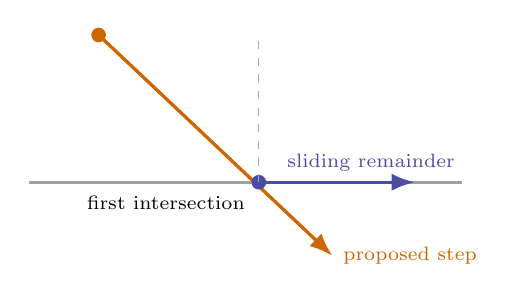
\begin{tikzpicture}[scale=1.1,>=Latex]
      \draw[very thick,gray!75] (-0.2,0) -- (4.8,0);
      \fill[orange!80!black] (0.6,1.7) circle (2.4pt);
      \draw[->,very thick,orange!80!black] (0.6,1.7) -- (3.3,-0.85) node[at end,right,font=\scriptsize]{proposed step};
      \fill[NavyBlue!70] (2.45,0) circle (2.4pt);
      \draw[->,very thick,NavyBlue!70] (2.45,0) -- (4.25,0) node[pos=0.72,above,font=\scriptsize]{sliding remainder};
      \draw[dashed,DarkGray] (2.45,0) -- (2.45,1.7);
      \node[font=\scriptsize,below left] at (2.4,-0.05) {first intersection};
    \end{tikzpicture}
    \raggedright
    \begin{alertblock}{Resolution matters}
    \small Large time steps can make collision searches expensive and obscure contact-time physics. Test step-size sensitivity for capture outcomes.
    \end{alertblock}
    {\scriptsize After every step, \code{Swarm.ib\_collision\_idx[i]} holds the index of the first mesh element agent $i$ struck in that step, or $-1$ if it struck none.\par}
  \end{column}
  \begin{column}{0.49\textwidth}
    \begin{description}
      \item[sliding] remove motion into the solid and project the remaining displacement along the boundary; recurse if another segment is encountered;
      \item[sticky] stop at first contact for that step (backed off the surface by a tiny $\varepsilon$, recorded velocity $=0$); model persistent attachment with agent state;
      \item[\code{None}] ignore immersed meshes;
      \item[\code{'default'}] use the Swarm's \code{ib\_condition} (default \code{'sliding'}).
    \end{description}
  \end{column}
\end{columns}
\sourcecredit{Schematic: instructor's course notes; collision rules from \code{planktos/\_ibc.py} and \code{Swarm.move}, commit \code{a1c2128}.}
\end{frame}

% 23
\begin{frame}{Moving meshes and sticky encounters}
\begin{columns}[T,onlytextwidth]
  \begin{column}{0.44\textwidth}
    \begin{itemize}
      \item The current code linearly interpolates supported 2D mesh vertices between stored times.
      \item Collision handling accounts for mesh motion over the step.
      \item A user state variable can turn a one-step sticky contact into persistent settlement or capture.
    \end{itemize}
    \begin{block}{Current limitation}
      FTLE calculations can respect static immersed boundaries, but moving meshes are not supported in that diagnostic.
    \end{block}
  \end{column}
  \begin{column}{0.52\textwidth}
    \centering
    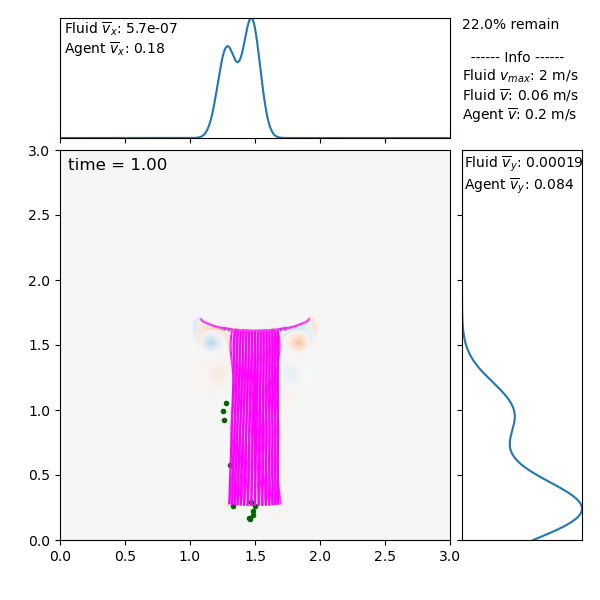
\includegraphics[height=0.60\textheight]{repo-moving-boundary-sticky.png}
  \end{column}
\end{columns}
\sourcecredit{Planktos documentation image \code{docs/\_static/ib2d\_mvbnd\_sticky.png} (commit \code{a1c2128}, GPLv3).}
\end{frame}

% 24
\begin{frame}{Visualization and population summaries}
\begin{columns}[c,onlytextwidth]
  \begin{column}{0.37\textwidth}
    \scriptsize
    \begin{itemize}
      \item \code{plot} gives snapshots; \code{plot\_all} makes animations.
      \item Position histories export to CSV, or to VTK point data (PolyData) for ParaView/VisIt; \code{save\_data} writes \code{shared\_props} to .npz and \code{props} to JSON (plus position history and current velocity/acceleration as CSV; \code{props\_history} is not saved).
      \item Vorticity or velocity may appear behind the agents.
      \item Marginal Gaussian KDEs summarize position distributions (SciPy \code{gaussian\_kde}; Scott's bandwidth factor by default).
    \end{itemize}
    \begin{alertblock}{KDE is an estimate}
      \scriptsize Bandwidth and boundary bias can change the apparent concentration; report the estimator settings.
    \end{alertblock}
  \end{column}
  \begin{column}{0.60\textwidth}
    \centering
    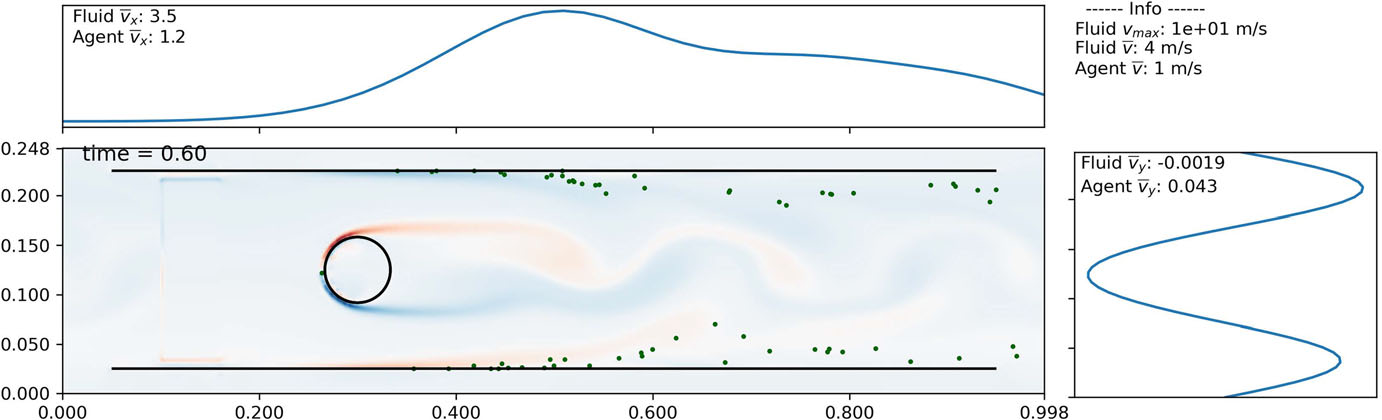
\includegraphics[width=\textwidth]{bmb2022-fig4-ib2d-kde.png}
  \end{column}
\end{columns}
\sourcecredit{Image: \href{https://doi.org/10.1007/s11538-022-01027-1}{Strickland et al. (2022), Fig. 4}, \emph{Bull.\ Math.\ Biol.}\ 84:72; educational reproduction (article not openly licensed).}
\end{frame}

% 25
\begin{frame}{FTLE: sensitivity of a deterministic flow map}
For a deterministic map $\bm\Phi_{t_0}^{T}$ with end time $T$ and integration duration $\tau=T-t_0$, define
\[
  \bm C=(D\bm\Phi)^T D\bm\Phi,
  \qquad
  \sigma_{t_0}^{\tau}(\XX_0)=\frac{1}{\tau}\ln\sqrt{\lambda_{\max}(\bm C)}.
\]
\begin{itemize}
  \item FTLE measures finite-time separation of initially nearby trajectories. Note $\ln\sqrt{\lambda_{\max}}=\tfrac12\ln\lambda_{\max}$: $\sqrt{\lambda_{\max}}$ is the largest stretch factor of an infinitesimal ball.
  \item Ridges may indicate candidate repelling transport structures, but ridge identification and LCS interpretation require care. Forward-time ridges $\rightarrow$ candidate repelling structures; backward-time ridges $\rightarrow$ attracting; \code{backward=True} is tracer-only in the current API.
  \item The diagnostic assumes independent deterministic agent dynamics on the initial-condition grid; ordinary stochastic realizations do not define a single smooth flow map.
\end{itemize}
\sourcecredit{Definition and scope: Strickland et al. (2022), Sections 2.1 and 4.2; current API documentation. FTLE/LCS background: Shadden et al. (2005); Haller (2015).}
\end{frame}

% 25b
\begin{frame}{FTLE in Planktos: what the implementation computes}
\begin{itemize}
  \item Agents are seeded on a grid (\code{grid\_dim}); $D\bm\Phi$ is approximated by central differences of the end positions, one-sided where a neighbor is masked.
  \item Planktos normalizes by the time actually integrated (changelog 1.0.3): at each grid point, $\tau$ is cut short to the last time before any finite-difference neighbor left the domain.
  \item In Planktos, forward-time FTLE can use tracers, selected ODEs, or deterministic custom behavior; backward-time support is more restricted.
  \item \code{T} is the end time (despite the docstring's ``integration time''); the call requires \code{T > t0}. With \code{backward=True} the map runs from \code{t0} back to \code{2*t0-T}.
  \item \code{FTLE\_largest} uses $\lambda_{\max}$; \code{FTLE\_smallest} uses $\lambda_{\min}$ of the same forward map (a contraction rate, not backward-time FTLE).
  \item Static immersed meshes are respected (sliding projection); moving meshes are refused.
\end{itemize}
\sourcecredit{Implementation: \code{Environment.calculate\_FTLE}, \code{planktos/\_environment.py}, commit \code{a1c2128}; \code{changelog.txt}, v1.0.3.}
\end{frame}

% 26
\begin{frame}{FTLE can reveal behavior-dependent transport barriers}
\begin{columns}[T,onlytextwidth]
  \begin{column}{0.66\textwidth}
    \centering
    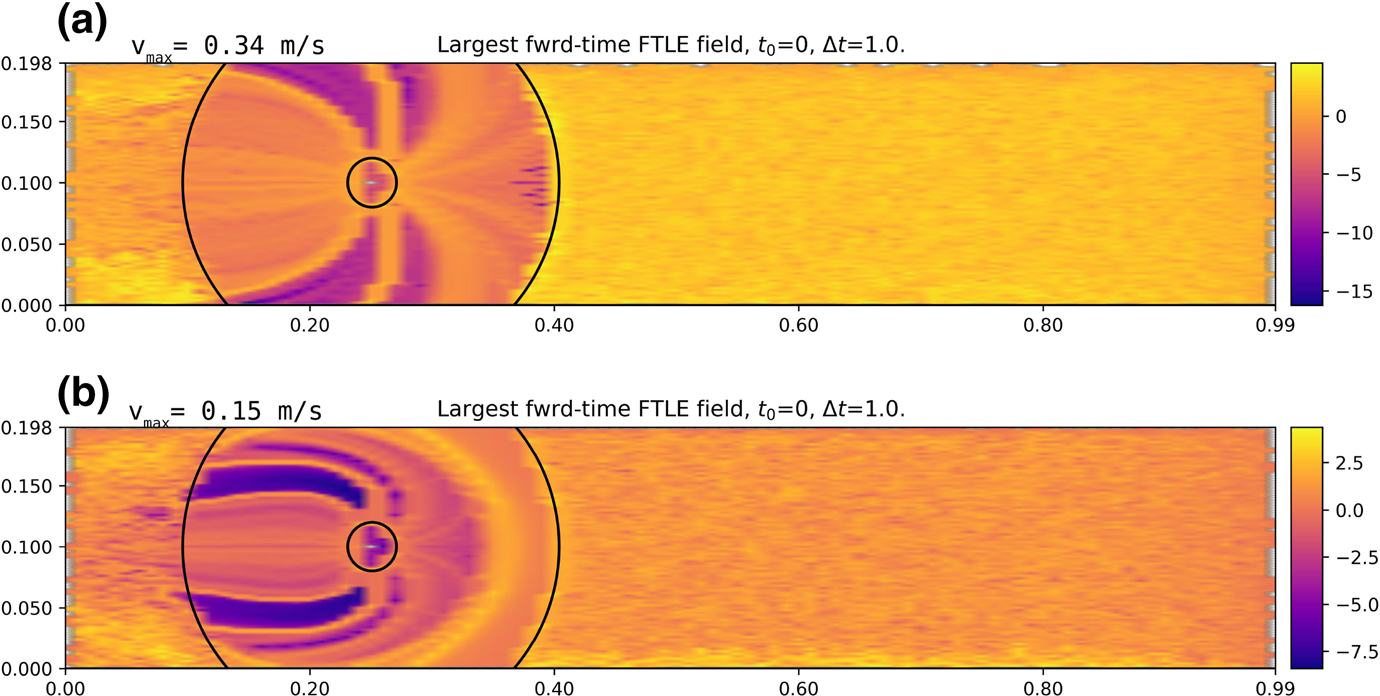
\includegraphics[width=\textwidth]{bmb2022-fig5-ftle.png}
  \end{column}
  \begin{column}{0.30\textwidth}
    \small
    Parasitoid-wasp agents fly toward a detected target cylinder in left-to-right flow.
    \begin{itemize}
      \item Faster active flight makes success primarily detection-limited.
      \item Slower active flight introduces a transport barrier inside the detection radius.
    \end{itemize}
  \end{column}
\end{columns}
\sourcecredit{Image and interpretation: \href{https://doi.org/10.1007/s11538-022-01027-1}{Strickland et al. (2022), Fig. 5}, \emph{Bull.\ Math.\ Biol.}\ 84:72; educational reproduction (article not openly licensed).}
\end{frame}

% 27
\begin{frame}{Collective rules can interact strongly with flow}
\begin{columns}[T,onlytextwidth]
  \begin{column}{0.68\textwidth}
    \centering
    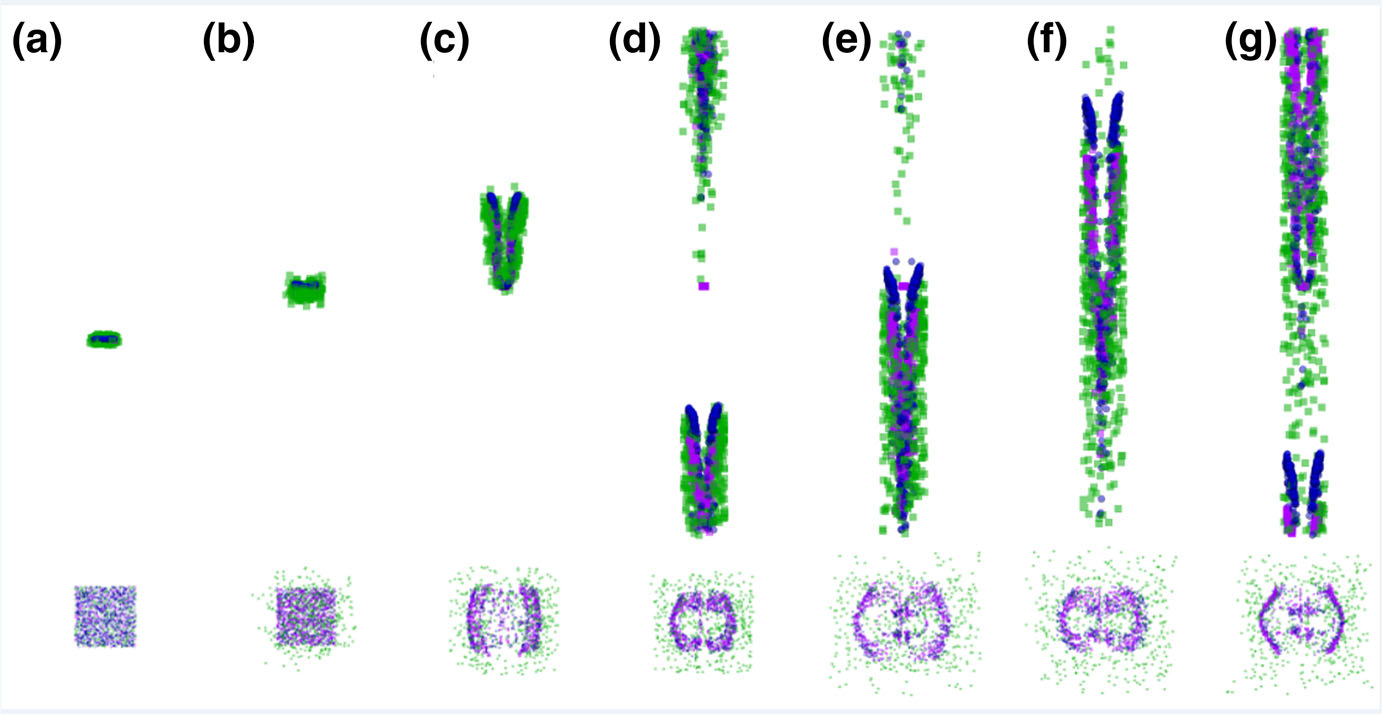
\includegraphics[width=\textwidth]{bmb2022-fig9-vicsek.png}
  \end{column}
  \begin{column}{0.28\textwidth}
    \small
    A Vicsek-type alignment model (Vicsek et al.\ 1995: each agent adopts its neighbors' mean heading plus noise) in periodic cylinder flow produces coherent, directional structure. Passive and Brownian agents in the same flow provide distinct baselines.
    \begin{block}{Lesson}
      A behavior calibrated in still fluid need not produce the same spatial statistics in a heterogeneous flow.
    \end{block}
  \end{column}
\end{columns}
\sourcecredit{Image: \href{https://doi.org/10.1007/s11538-022-01027-1}{Strickland et al. (2022), Fig. 9}, \emph{Bull.\ Math.\ Biol.}\ 84:72; educational reproduction (article not openly licensed).}
\end{frame}

% 28
\begin{frame}{Application: flow through a gorgonian hierarchy}
\begin{columns}[T,onlytextwidth]
  \begin{column}{0.56\textwidth}
    \centering
    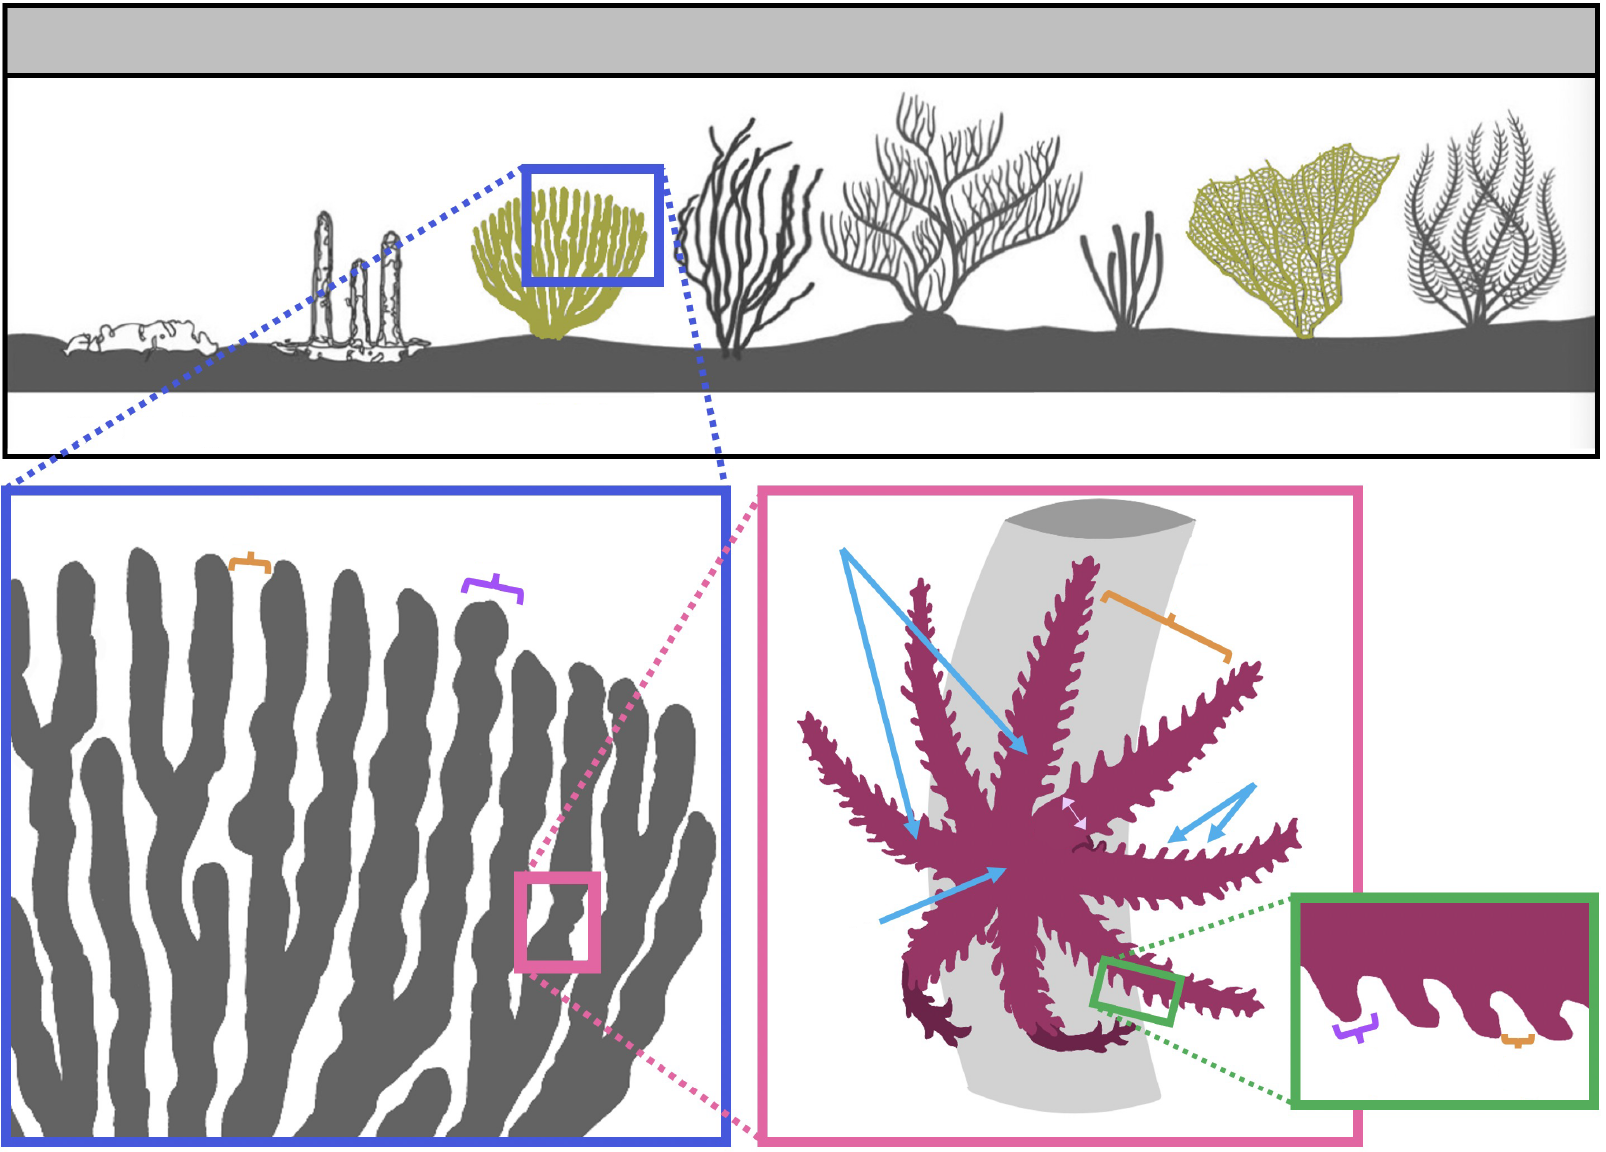
\includegraphics[width=\textwidth]{jeb2023-fig1-gorgonian-scales.png}
  \end{column}
  \begin{column}{0.40\textwidth}
    \small
    Gorgonians present nested flow filters:
    \begin{itemize}
      \item colony and branches;
      \item polyps and tentacles;
      \item pinnules on the tentacles.
    \end{itemize}
    At each level, gap-to-diameter ratio and Reynolds number set leakiness. Branches and tentacles can span a leaky-to-solid transition; pinnules mostly impeded flow in the tested range.
  \end{column}
\end{columns}
\sourcecredit{Image: \href{https://doi.org/10.1242/jeb.244520}{Hamlet et al. (2023), Fig. 1} (adapted from Kupfner Johnson \& Hallock, 2020), CC BY 4.0.}
\end{frame}

% 29
\begin{frame}{From CFD to a Planktos capture experiment}
\begin{columns}[c,onlytextwidth]
  \begin{column}{0.61\textwidth}
    \centering
    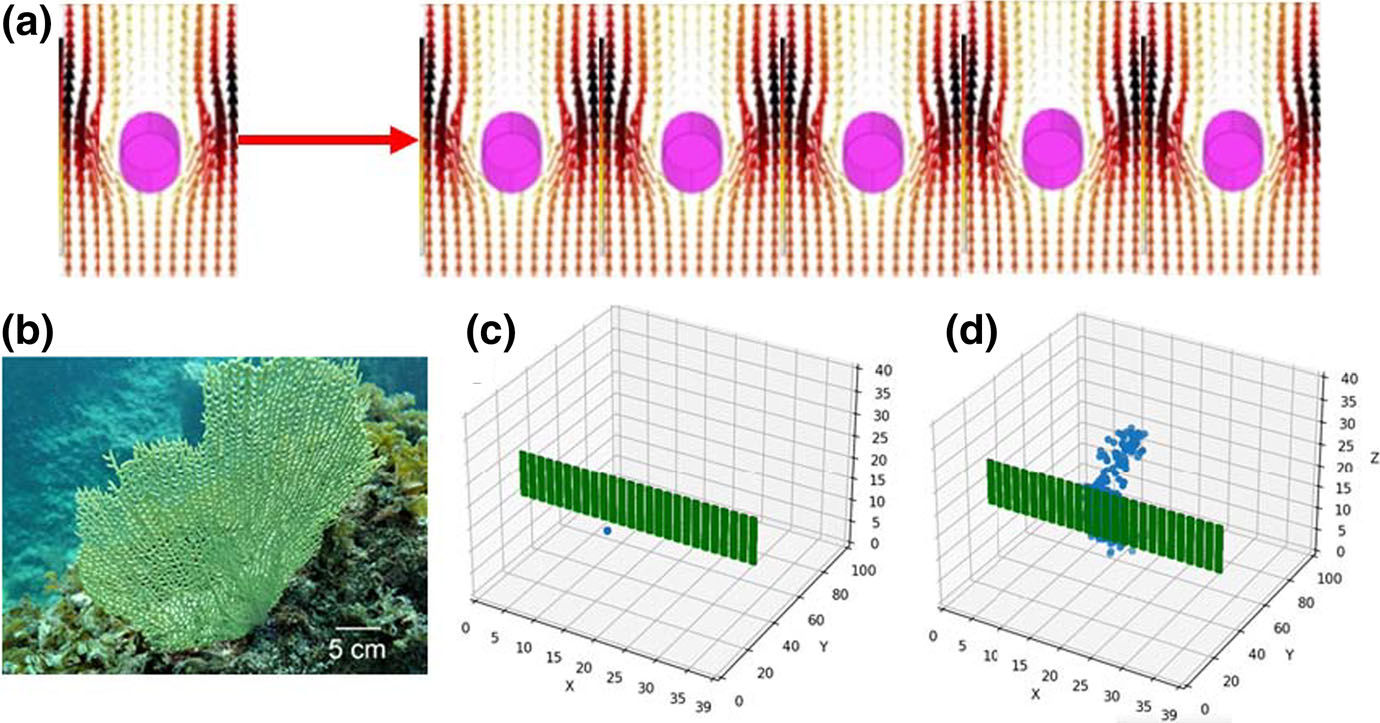
\includegraphics[width=\textwidth]{bmb2022-fig8-seafan-capture.png}
  \end{column}
  \begin{column}{0.35\textwidth}
    \small
    \begin{enumerate}
      \item Solve steady flow around one cylinder with periodic lateral boundaries.
      \item Tile the field to represent an array of idealized branches.
      \item Release agents upstream.
      \item Add unbiased Brownian motion to local fluid advection.
      \item Treat contact with a cylinder as capture.
    \end{enumerate}
  \end{column}
\end{columns}
\sourcecredit{Image: \href{https://doi.org/10.1007/s11538-022-01027-1}{Strickland et al. (2022), Fig. 8}, \emph{Bull.\ Math.\ Biol.}\ 84:72; educational reproduction (article not openly licensed).}
\end{frame}

% 30
\begin{frame}{The 2023 gorgonian capture study}
\begin{columns}[c,onlytextwidth]
  \begin{column}{0.42\textwidth}
    \centering
    
\includegraphics[width=\textwidth]{jeb2023-fig6a-polyp-array.png}
  \end{column}
  \begin{column}{0.54\textwidth}
    \small
    \begin{itemize}
      \item COMSOL fields were tiled into a $3.6\times10\times4.0$ cm domain containing an idealized periodic branch array.
      \item Each case used 1000 agents and 100 repeated simulations.
      \item Agents followed local flow plus unbiased Brownian motion; cylinder contact counted as capture.
      \item For $\mathrm{Re}_b=8$, capture peaked near $G_b/D_b=1$; for $\mathrm{Re}_b=1$, it peaked near $G_b/D_b=1.75$.
      \item Capture fell when gaps were too narrow or too wide: morphology controlled both delivery and residence near the boundary.
    \end{itemize}
  \end{column}
\end{columns}
\sourcecredit{Image: \href{https://doi.org/10.1242/jeb.244520}{Hamlet et al. (2023), Fig. 6A}, CC BY 4.0; results from Fig. 7.}
\end{frame}

% 31
\begin{frame}{Interpret the application within its assumptions}
\begin{columns}[T,onlytextwidth]
  \begin{column}{0.48\textwidth}
    \textbf{What the model supports}
    \begin{itemize}
      \item capture depends jointly on morphology and flow regime;
      \item an intermediate gap can balance transport through the array with time near the capture surface;
      \item agent-based simulation connects resolved flow to encounter statistics.
    \end{itemize}
  \end{column}
  \begin{column}{0.48\textwidth}
    \textbf{What remains outside it}
    \begin{itemize}
      \item deformable or swaying colonies and fully coupled FSI;
      \item finite-size prey and hydrodynamic feedback;
      \item adhesion force, contact duration, and post-contact escape;
      \item unsteady environmental forcing and whole-colony scale separation.
    \end{itemize}
  \end{column}
\end{columns}
\begin{block}{Modeling principle}
``Contact equals capture'' is an operational rule whose biological adequacy must be tested, not a universal law.
\end{block}
\sourcecredit{Caveats: Hamlet et al. (2023), Discussion.}
\end{frame}

% 32
\begin{frame}{Takeaways and source trail}
\begin{itemize}
  \item Planktos couples \textbf{prescribed flow}, \textbf{agent behavior}, and \textbf{immersed geometry} without agent-to-fluid feedback.
  \item \code{Environment} owns Eulerian fields and geometry; \code{Swarm} owns vectorized Lagrangian state and behavior.
  \item Flow interpolation, collision rules, and stochastic conventions are part of the mathematical model and should be verified explicitly.
  \item KDE describes an ensemble distribution; FTLE describes sensitivity of a deterministic finite-time map. They answer different questions.
  \item The gorgonian study shows the intended workflow: CFD $\rightarrow$ trajectory model $\rightarrow$ capture statistics $\rightarrow$ qualified biological inference.
\end{itemize}
\vspace{0.3em}
{\scriptsize
\textbf{Primary sources:}
\href{https://doi.org/10.1007/s11538-022-01027-1}{Strickland et al., \emph{Bull. Math. Biol.} 84:72 (2022)};
\href{https://doi.org/10.1242/jeb.244520}{Hamlet et al., \emph{J. Exp. Biol.} 226, jeb244520 (2023), CC BY 4.0}.\\[2pt]
\textbf{Software source audited:}
\href{https://github.com/mountaindust/Planktos}{Planktos}, version 1.0.3, commit \code{a1c2128} (2026-08-19), GPLv3.
}
\end{frame}

% 33
\begin{frame}{References}
\footnotesize
\begin{itemize}\itemsep3pt
  \item W. C. Strickland, N. A. Battista, C. L. Hamlet, and L. A. Miller, ``Planktos: an agent-based modeling framework for small organism movement and dispersal in a fluid environment with immersed structures,'' \emph{Bull. Math. Biol.} 84 (2022), 72, \href{https://doi.org/10.1007/s11538-022-01027-1}{doi:10.1007/s11538-022-01027-1}. Source of the deck's framing and of Figs.~4, 5, 8, 9 (reproduced for education; not openly licensed).
  \item C. L. Hamlet, W. C. Strickland, N. Battista, and L. A. Miller, ``Multiscale flow between the branches and polyps of gorgonians,'' \emph{J. Exp. Biol.} 226(5) (2023), jeb244520, \href{https://doi.org/10.1242/jeb.244520}{doi:10.1242/jeb.244520}. CC BY 4.0; Figs.~1 and 6A reproduced, Fig.~7 results summarized.
  \item W. C. Strickland \emph{et al.}, \emph{Planktos} agent-based modeling framework, v1.0.3, commit \code{a1c2128} (2026-08-19), GPLv3, \url{https://github.com/mountaindust/Planktos}; documentation \url{https://planktos.readthedocs.io}. Source of the API statements, the example listing (\code{examples/ex\_sticky\_seafan\_3d.py}), and the \code{docs/\_static} images.
  \item S. Kupfner Johnson and P. Hallock, ``A review of symbiotic gorgonian research in the western Atlantic and Caribbean with recommendations for future work,'' \emph{Coral Reefs} 39 (2020), 239--258, \href{https://doi.org/10.1007/s00338-020-01891-0}{doi:10.1007/s00338-020-01891-0}. Original source adapted in Hamlet et al.\ (2023), Fig.~1.
  \item M. R. Maxey and J. J. Riley, ``Equation of motion for a small rigid sphere in a nonuniform flow,'' \emph{Phys. Fluids} 26 (1983), 883--889, \href{https://doi.org/10.1063/1.864230}{doi:10.1063/1.864230}.
  \item G. Haller and T. Sapsis, ``Where do inertial particles go in fluid flows?'' \emph{Physica D} 237 (2008), 573--583, \href{https://doi.org/10.1016/j.physd.2007.09.027}{doi:10.1016/j.physd.2007.09.027}.
\end{itemize}
\end{frame}

% 34
\begin{frame}{References (continued)}
\footnotesize
\begin{itemize}\itemsep3pt
  \item T. Vicsek, A. Czir\'ok, E. Ben-Jacob, I. Cohen, and O. Shochet, ``Novel type of phase transition in a system of self-driven particles,'' \emph{Phys. Rev. Lett.} 75 (1995), 1226--1229, \href{https://doi.org/10.1103/PhysRevLett.75.1226}{doi:10.1103/PhysRevLett.75.1226}.
  \item S. C. Shadden, F. Lekien, and J. E. Marsden, ``Definition and properties of Lagrangian coherent structures from finite-time Lyapunov exponents in two-dimensional aperiodic flows,'' \emph{Physica D} 212 (2005), 271--304, \href{https://doi.org/10.1016/j.physd.2005.10.007}{doi:10.1016/j.physd.2005.10.007}.
  \item G. Haller, ``Lagrangian coherent structures,'' \emph{Annu. Rev. Fluid Mech.} 47 (2015), 137--162, \href{https://doi.org/10.1146/annurev-fluid-010313-141322}{doi:10.1146/annurev-fluid-010313-141322}. Caveats on reading FTLE ridges as LCS.
  \item P. E. Kloeden and E. Platen, \emph{Numerical Solution of Stochastic Differential Equations}. Springer, 1992, \href{https://doi.org/10.1007/978-3-662-12616-5}{doi:10.1007/978-3-662-12616-5}. Euler--Maruyama and Milstein schemes and their strong orders.
  \item J. R. Dormand and P. J. Prince, ``A family of embedded Runge--Kutta formulae,'' \emph{J. Comput. Appl. Math.} 6 (1980), 19--26, \href{https://doi.org/10.1016/0771-050X(80)90013-3}{doi:10.1016/0771-050X(80)90013-3}. The RK45 pair behind SciPy's \code{solve\_ivp}.
\end{itemize}
\end{frame}

% 35
\begin{frame}{References (continued)}
\footnotesize
\begin{itemize}\itemsep3pt
  \item D. W. Scott, \emph{Multivariate Density Estimation}. Wiley, 1992, \href{https://doi.org/10.1002/9780470316849}{doi:10.1002/9780470316849}. Scott's KDE bandwidth factor.
  \item N. A. Battista, W. C. Strickland, and L. A. Miller, ``IB2d: a Python and MATLAB implementation of the immersed boundary method,'' \emph{Bioinspir. Biomim.} 12 (2017), 036003, \href{https://doi.org/10.1088/1748-3190/aa5e08}{doi:10.1088/1748-3190/aa5e08}. Source format of the IB2d flow and mesh data.
\end{itemize}
\begin{punchbox}
\footnotesize The flow-and-agents cartoon, the architecture diagram, and the collision sketch were drawn for these notes (TikZ). Planktos issue cited on the immersed-geometry slide: \url{https://github.com/mountaindust/Planktos/issues/75}.
\end{punchbox}
\end{frame}

\end{document}
